%%%%%%%%%%%%%%%%%%%%%%%%%%%%%%%%%%%%%%%%%
% University/School Laboratory Report
% LaTeX Template
% Version 3.1 (25/3/14)
%
% This template has been downloaded from:
% http://www.LaTeXTemplates.com
%
% Original author:
% Linux and Unix Users Group at Virginia Tech Wiki 
% (https://vtluug.org/wiki/Example_LaTeX_chem_lab_report)
%
% License:
% CC BY-NC-SA 3.0 (http://creativecommons.org/licenses/by-nc-sa/3.0/)
%
%%%%%%%%%%%%%%%%%%%%%%%%%%%%%%%%%%%%%%%%%

%----------------------------------------------------------------------------------------
%	PACKAGES AND DOCUMENT CONFIGURATIONS
%----------------------------------------------------------------------------------------

\documentclass{article}

\usepackage[version=3]{mhchem} % Package for chemical equation typesetting
\usepackage{siunitx} % Provides the \SI{}{} and \si{} command for typesetting SI units
\usepackage{graphicx} % Required for the inclusion of images
\usepackage{natbib} % Required to change bibliography style to APA
\usepackage{amsmath} % Required for some math elements 
\usepackage{hyperref}

\setlength\parindent{0pt} % Removes all indentation from paragraphs

\renewcommand{\labelenumi}{\alph{enumi}.} % Make numbering in the enumerate environment by letter rather than number (e.g. section 6)

%\usepackage{times} % Uncomment to use the Times New Roman font

%----------------------------------------------------------------------------------------
%	DOCUMENT INFORMATION
%----------------------------------------------------------------------------------------

\title{Jojo2Space CR01-072014\\Rock Launch Summary Report (for English majors)} % Title

\author{Charles \textsc{Hathaway} \\Ranjani \textsc{Sargunaraj}} % Author name

\date{\today} % Date for the report

\begin{document}

\maketitle % Insert the title, author and date

% If you wish to include an abstract, uncomment the lines below
% \begin{abstract}
% Abstract text
% \end{abstract}

%----------------------------------------------------------------------------------------
%	SECTION 1
%----------------------------------------------------------------------------------------

\section{Objective}

The objective of this report is to summarize, in very basic terms, the process and related calculations that can go into a simple model rocket launch.
Although there are some algorithms, the goal of this paper is to be understandable by people without a significant math background (for example, English majors).

The first section will talk about the procedure and process required to assemble and launch the rocket.
The most important takeaway is the needed materials, which are not clearly stated on the rocket's product page.

The second section will be an abstract discussion about the relationship between Newton's Laws and our rocket.
It will conclude with a numerical analysis of the rocket launch, solving for a few pieces of data.
 
\section{Procedure and Materials}

\subsection{Bill of Materials}

To perform a simple rocket launch, we used the following commercial-over-the-shelf products:

\begin{itemize}
 \item Estes 1469 Tandem-X Launch Set \url{http://www.amazon.com/gp/product/B002VLP67S/ref=oh_aui_detailpage_o01_s00?ie=UTF8&psc=1}
 \begin{itemize}
	 \item This set includes 2 rockets; the second rocket requires much more assembly. We only used the first
	 \item This set also contains the launch pad
 \end{itemize}
 \item Estes B4-2 Engine Pack (3-Each) \url{http://www.amazon.com/gp/product/B000QV08F0/ref=oh_aui_detailpage_o00_s00?ie=UTF8&psc=1}
 \item Estes 2274 Recovery Wadding \url{http://www.amazon.com/gp/product/B0006NAQ6O/ref=oh_aui_detailpage_o02_s00?ie=UTF8&psc=1}
 \item CVS Super Glue Gel 2-Pack \url{http://www.cvs.com/shop/product-detail/CVS-Super-Glue-Gel-2-Pack?skuId=904326}
 \begin{itemize}
	 \item This kind of glue isn't required, but it worked. You need a glue that can bond to both plastic and cardboard.
 \end{itemize}
 \item 9V "Square" battery
 \item Philips head screwdriver
 \item Protractor \url{http://www.cvs.com/shop/product-detail/Caliber-Protractor?skuId=138038}
 \item 25' tape measure
 \item Stopwatch (we used a cell phone)
 \item 2-3 people
 \item Notebook, pencil
 \item (Optional) Acrylic-based paint and paint brushes
 \begin{itemize}
	 \item Although this wasn't perfect, it did stick to the surface of the rocket. Spray paint and stencils would probably work better
 \end{itemize}
\end{itemize}

\subsection{Procedure}

Assemble the rocket and launch pad as per the instructions included with the rocket.
When assembled and ready to launch (parachute in, engine in), weigh the rocket!

Find a large open field, and begin the fun!

Place the launch pad in the center of the field.
Measure out from it (using the tape measure) about 100ft in a straight line (you can use 2 people for this!)
This is where the person will stand while measure the angle the rocket goes to that we will use to determine the height.

Uncoil the launch button, insert the battery.
When launching the rocket, you should have people doing the following things;
\begin{itemize}
	\item Using the protractor, "follow" the rocket with the arm until it reaches it's apex (the parachute will blow). Record this angle as $\theta_{rocket}$
	\begin{itemize}
		\item The protractor should be held at level angle; the arm get's rotated to track the rocket
		\item Measure and record the height that the person is holding the rocket as $d_1$
	\end{itemize}
	\item Using the stopwatch, measure to time it takes to reach it's apex. Record this value as $t_{rocket}$
	\item Launch the rocket (requires countdown)
	\item Record video of the launch (optional)
\end{itemize}

Repeat this experiment until you run out of engines (or your rocket blows up)

\section{Discussion}

\subsection{Newton's Laws}

Every has heard the of Newton's three laws (if you haven't, don't fret! We will recap them here!).
They are of interest to us because they help explain how the rocket works, without the need of calculus.

\begin{enumerate}
	\item "An object at rest stays at rest and an object in motion stays in motion unless acted upon by an outside force". This is paraphrased a bit, but still not too hard.
	\begin{itemize}
		\item Something won't move unless it is pushed
		\item Something won't stop unless something stops it. Most things stop because of friction
	\end{itemize}
	\item The second law is more tricky, but basically means that an objects velocity (speed in a direction) is changed due it's acceleration
	\begin{itemize}
		\item Wikipedia discusses this using calculus, which is a pain.
		\item Think of it this way; if a car is moving forward and you press the gas, it starts to move forward faster. The velocity of the car increases every moment that you hold down the gas, as long as you keep it accelerating
		\item Remember gravity? Gravity pulls things together, most notably it pulls things down to Earth. When you throw something (or launch it), you accelerate it very quickly and it goes up. Gravity pulls it down, lowering it's velocity, until it reaches a velocity of 0, then it starts to fall back down (getting faster and faster!)
	\end{itemize}
	\item "For every action there is an equal and opposite reaction"
	\begin{itemize}
		\item This is not actually very important to us :). But it is cool! (when you launch the rocket, you push the Earth down... So why don't you feel the earth moving?)
	\end{itemize}
\end{enumerate}

\subsubsection{Take aways}

Newton's first law is inertia. Inertia is the mass of an object times it's speed.

Newton's second law is about acceleration (which is just how the speed is changing by).

Newton's third law is about why perpetual energy machines can't exist.

\subsection{How does this relate to the Rocket?}

We start with the rocket sitting on the launch bad, moving at 0m/s.
When we ignite the engine, it starts to accelerate (but how fast?? that is why we do math).
Once the engine burns up, the rocket has a velocity of something, but now has a negative acceleration (gravity!).
So the rocket slows down, eventually stops for a split moment, then starts falling back to earth.

The point where the rocket stops is how high it gets.

\subsection{The Mathy Bit}

Ok, so now we get to do the math things.
Our goal is to figure out:
\begin{itemize}
	\item How high the rocket went
	\item How high a different rocket would go with the same engine
	\begin{itemize}
		\item For example, the second rocket in the pack
	\end{itemize}
\end{itemize}

\subsubsection{Measuring Height}

In order to measure the height, we are going to take advantage of the properties of right triangles.
Recall from the way-way-back machine the SOHCAHTOA rule (sin = opposite over hypotenuse, cos = adjacent over hypotenuse, tan = opposite over adjacent).

Figure \ref{triangle} shows how we setup the launch.
The observer with the protractor is recording the angle the rocket reaches at $\theta_{rocket}$ while standing 100ft (30.48 meters) away from the launch pad.
Using this value, we calculate $d_2$, add $d_1$, and then we will know how the rocket went. \\

$d_2=100ft*tan(\theta_{rocket})$

$height ~of ~rocket=d_1+d_2$ \\

Make sure you're using degrees in your calculator!

\subsubsection{Predicting height of the next rocket}

To predict the height of the next rocket, we need to know how much "force" the engine provided.
Force is the total acceleration.
Finding this value can be very hard, unless we cheat.

We know how high the rocket went, we know how much the rocket weighed, and we know how much force it took to get there (gravity!).
To determine the force provided by the engine, we simply multiply the weight of the rocket by the height by the force of gravity here on Earth.
Units are important!
Convert all your measurements to the metric system;
\begin{itemize}
	\item (m) Weight should be in kg
	\item (h) Height should be in meters
	\item (a) Acceleration (gravity) is $9.81 \frac{m}{s^2}$
\end{itemize}

To find the force (in Newtons... not important), simply multiply all your values together. \\

$F=m*h*a$ \\

To determine how high the next rocket will go, we just change the mass, and solve for h.
So... \\

$h=\frac{F}{m*a}$

\begin{figure}[h]
\begin{center}
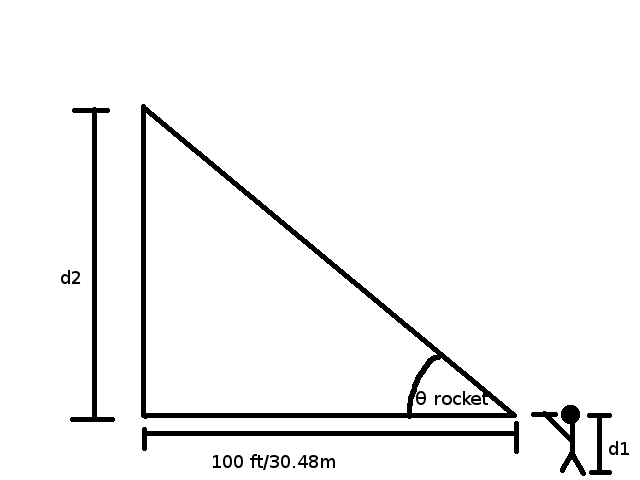
\includegraphics[width=0.65\textwidth]{triangle}
\caption{Diagram of rocket launch}
\label{triangle}
\end{center}
\end{figure}

\section{Actual results}

Unfortunately, we only got one good launch.
One launch we just recorded with the camera, the other had too much wind. \\

$m=0.116kg$

$\theta_{rocket}=79 degrees$

$d_1=70"=1.778m$ \\

So our results are... \\

$d_2=100ft*tan(\theta_{rocket})=$
$30.48m*tan(79 degrees)=156.81m$

$h=156.81m+1.778m=158.59m=520.308ft$

$F=m*g*h=0.116kg*9.81\frac{m}{s^2}*158.59m=180.4690764N$


%----------------------------------------------------------------------------------------


\end{document}